%!TEX root = draft.tex
\section{Scaling} \label{sec:scaling}
In this section we present results that show the scalability of our algorithms. All of our tests have been run on the Stampede cluster at Texas Advanced Computing Center (TACC) where we are limited to $4096$ cores at most. Each node of Stampede has 2 eight-core Xenon E5-2680 processors clocked at 2.7 GHz with 32 GB of DDR3-1600 MHz memory and interconnected using an InfiniBand network card. Unless mentioned otherwise, in all the tests we have used all 16 cores of every node. Finally, in all cases we report the maximum wall time recorded using PETSc's logging interface which has a temporal resolution of roughly $0.1 \: \mu s$.

\subsection{Interpolation}
In this section we show results for a simple test to measure the scalability of the interpolation algorithm \ref{alg:interpolation}. The test consists of interpolating a function at a number of random points on a randomly refined octree in three dimensions. We consider two cases. A small test on a level 9 tree with roughtly 20M cells and 33M nodes and larger test on a level 13 tree with roughly 128M cells and 280M nodes. In both cases number of randomly generated points are chosen to be equal to the number of nodes and the stablized second-order interpolation of \cite{Min;Gibou:07:A-second-order-accur} was performed 10 times to smooth out possible timing fluctuations.

To simulate the effect of different CFL numbers, we generate the random points such that on each processor $\alpha$ percentage of them are located outside the processor boundary and thus will initiate communication. Scaling results are presented for $\alpha = 5 \%$ and $\alpha = 95\%$ for both small and large problems in figure \ref{fig:interpolation}. Excellent scaling is obtained for the small problem for $P = 16-512$ even when $95\%$ of interpolation points are remote to processors. For the larger problem, communication overhead prevents further scaling of algorithm beyond $4096$ processors when $\alpha = 95\%$. Note that for $\alpha = 5\%$, even though some sections of algorithm stop scaling, the overall algorithm still scales since the local work dominates the timing. This illustrates the effectiveness of non-blocking communication pattern in algorithm \ref{alg:interpolation}.

\begin{figure}[htbp]
	\begin{center}
		\subfigure[$N_G = 33$M, $\alpha = 5\%$]{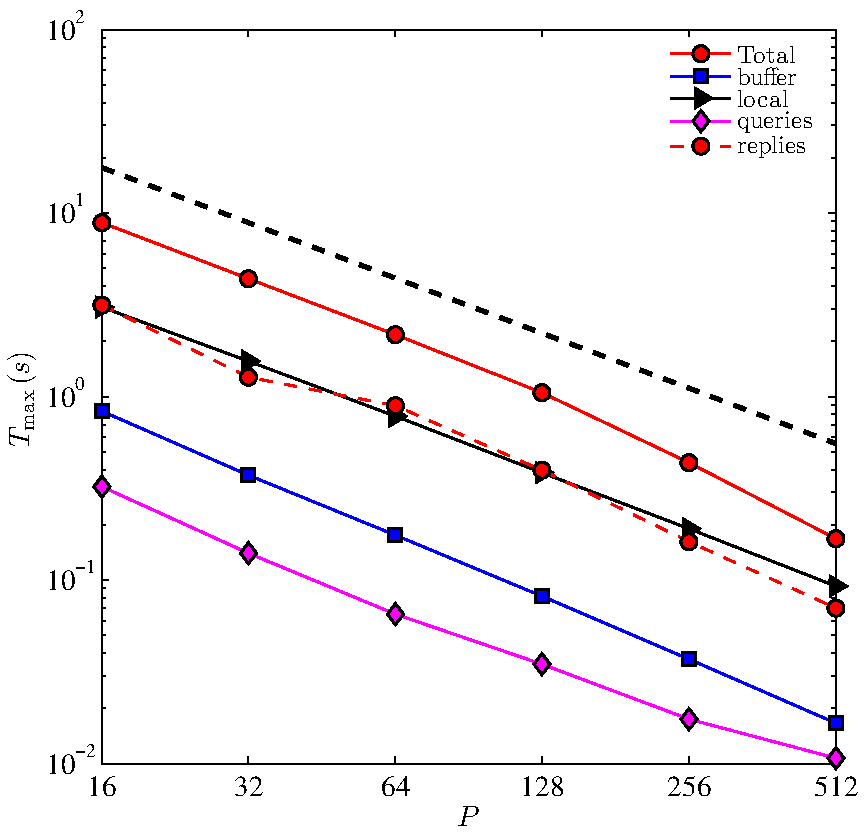
\includegraphics[width = 0.45 \textwidth] {figures/interpolation_small_05.pdf}}
		\subfigure[$N_G = 33$M, $\alpha = 95\%$]{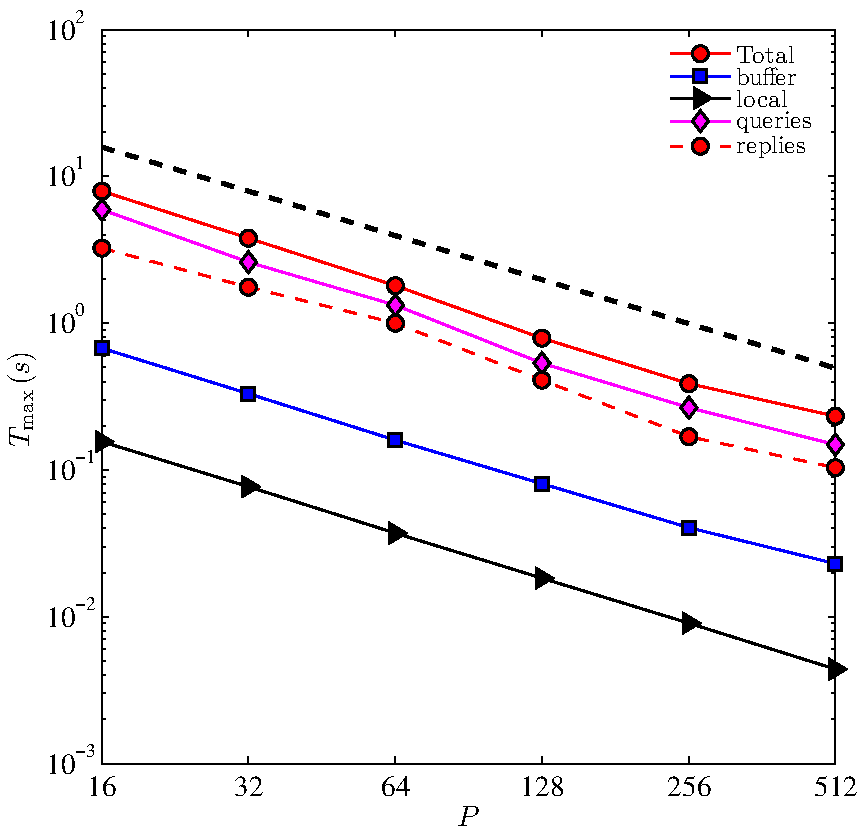
\includegraphics[width = 0.45 \textwidth] {figures/interpolation_small_95.pdf}}
		\\
		\subfigure[$N_G = 280$M, $\alpha = 5\%$]{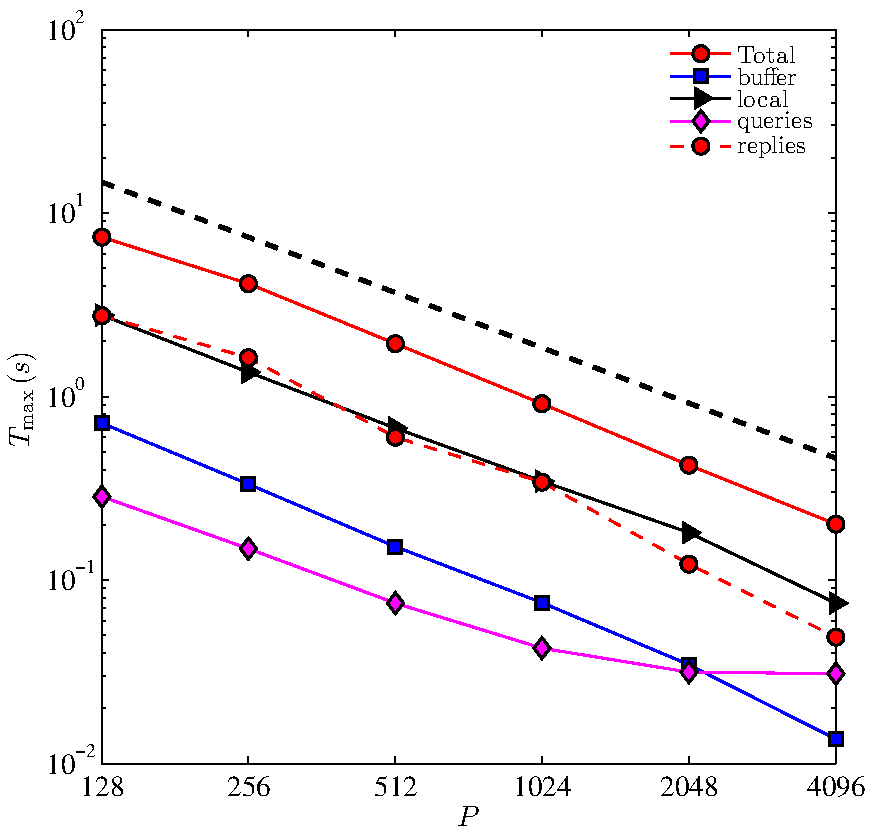
\includegraphics[width = 0.45 \textwidth] {figures/interpolation_large_05.pdf}}
		\subfigure[$N_G = 280$M, $\alpha = 95\%$]{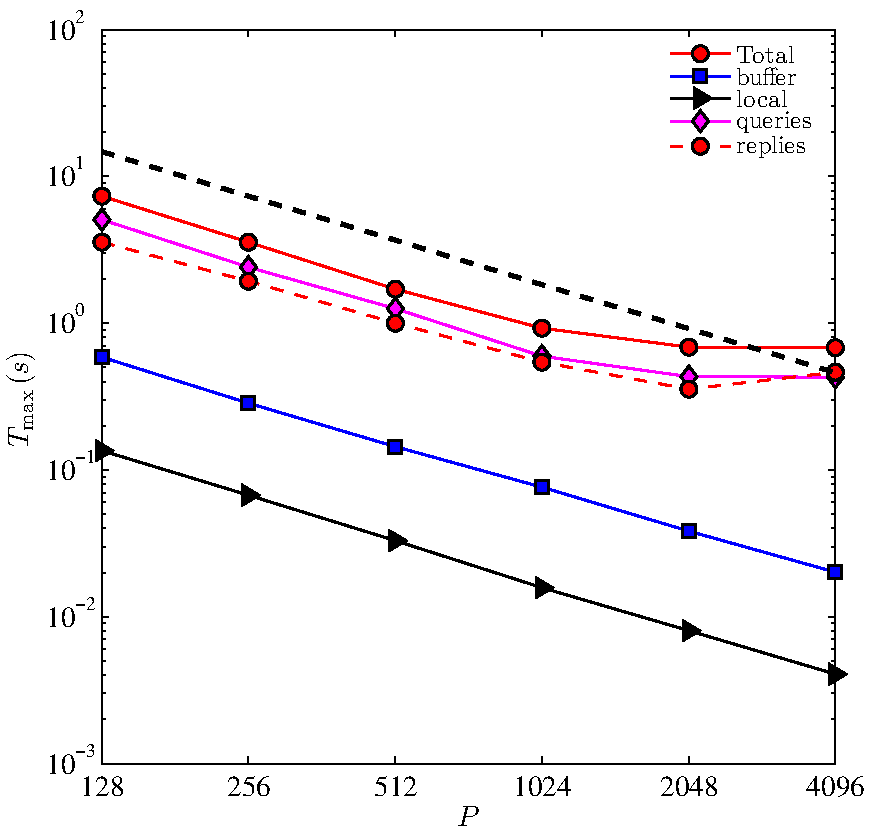
\includegraphics[width = 0.45 \textwidth] {figures/interpolation_large_95.pdf}}
	\end{center}
	\caption{Strong scaling of algorithm \ref{alg:interpolation} for several tests where $N_G$ denotes the number of random interpolation points (same as number of nodes in the octree) and $\alpha$ denotes the percentage of these points that are remote to each processor. Here ``Total'' represents the total time spent in the interpolation while ``buffer'', ``local'', ``queries'', and ``replies'' represent the the timing for different sections (c.f. algorithm \ref{alg:interpolation}). Results indicate excellent scaling for the small test (a-b) and for the large test when $\alpha = 5\%$ (c). For the extreme case (d) the algorithm stops scaling at $4096$ processors due to communication overhead.}
	\label{fig:interpolation}
\end{figure}

\subsection{Semi-Lagrangian}
To test the scalability of the Semi-Lagrangian algorithm \ref{alg:semi-lagrangian} we consider a slightly modified version of the Enright's rotation test \cite{Enright;Fedkiw;Ferziger;etal:02:A-Hybrid-Particle-Le}, i.e. we advect a sphere of radius 0.35 located at $(0.4, 0.4, 0.4)$ with a divergent free velocity field given by:
\bean
u(x,y,z) &=& 2\sin(\pi x)^2 \sin(2\pi y) \sin(2 \pi z), \\
v(x,y,z) &=& -\sin(\pi y)^2 \sin(2\pi x) \sin(2 \pi z),\\
w(x,y,z) &=& -\sin(\pi z)^2 \sin(2\pi x) \sin(2 \pi y). 
\eean
To understand the effect of CFLnumber on the scalability of the algorithm we perform one step of the Semi-Lagrangian algorithm for $\text{CFL} = 1$, $\text{CFL} = 10$, and $\text{CFL} = 100$. We also perform the test for two set of initial girds, a small grid with $l_\max = 10$ and a larger grid with $l_\max = 12$. After one advection step, each of these grids have approximately 15M and 255M nodes, respectively. 
\begin{table}[htbp]
	\begin{minipage}{.5\linewidth}
		\begin{center}
		\begin{tabular}{ccccccc}
			\hline
				CFL & 16 & 32 & 64 & 128 & 256 & 512 \\
				\hline
				1   & 2 & 2 & 3 & 3 & 3 & 3 \\
				10  & 3 & 3 & 3 & 3 & 3 & 3 \\
				100 & 6 & 6 & 6 & 6 & 6 & 6 \\
			\hline
		\end{tabular}
		\caption*{(a) $l_\max = 10$}
		\end{center}
	\end{minipage}%
	\begin{minipage}{.5\linewidth}
		\begin{center}
		\begin{tabular}{ccccccc}
			\hline
				CFL & 128 & 256 & 512 & 1024 & 2048 & 4096 \\
			\hline
				1   & 3 & 3 & 3 & 3 & 3 & 3 \\
				10  & 3 & 3 & 4 & 4 & 4 & 4 \\
				100 & 6 & 6 & 6 & 6 & 6 & 7 \\
			\hline
		\end{tabular}
		\caption*{(b) $l_\max = 12$}
		\end{center}
	\end{minipage}	
	\caption{Number of iterations required for grid construction in algorithm \ref{alg:semi-lagrangian} for the rotation test on a (a) level-10 and (b) level-12 octree with approximately 15M and 255M nodes, respectively. Note how the iteration count increases with the CFL number but is almost independent of number of processors. The slight dependence of iteration count on number of processors is most likely due to dependence of round-off errors on the number of processors. Nonetheless, close examination of generated octrees (data not shown) reveals that they are identical and independent of the number of processors used to perform the test.}
	\label{tab:semilagrangian}
\end{table}

Table \ref{tab:semilagrangian} illustrates the dependence of number of iterations required to build the grid; as the CFL is increased, interface travels a farther distance which necessitates more iterations to generate the grid. Note that the apparent dependence on the number processors is most likely due to round-off errors during the interpolation and/or backtracking step. Figures \ref{fig:semilagrangian_small} and \ref{fig:semilagrangian_large} illustrate the scalability of the algorithm for small and large problems, respectively. To enable meaningful comparisons between different CFL numbers and number of processors, the maximum time has been scaled to the number of iterations required for grid construction as reported in table \ref{tab:semilagrangian}. For both problems excellent scalability is observed for $\text{CFL} = 1$ and $\text{CFL} = 10$. The algorithm even shows good scalability when taken to the extreme, i.e. for $\text{CFL} = 100$.

An increase in the CFL number has two effects on the algorithm. First, a larger fraction of departure points land in domains of remote processors. Moreover, these points are potentially dispersed across a larger number of processors. This means both the number MPI messages and their volume increases for larger CFL numbers. Second, as more points are shipped to remote processors for interpolation, there is a greater chance that interpolation load is unbalanced across processors. This is specially true for regions of space in which streamlines cluster. Both factors contribute to decrease the scalability of the algorithm at larger CFL numbers. To shed more light on this, we have recorded a complete history of communication pattern in the interpolation step.

\begin{figure}[htbp]
	\begin{center}
		\subfigure[Semi-Lagrangian, $\text{CFL} = 1$]{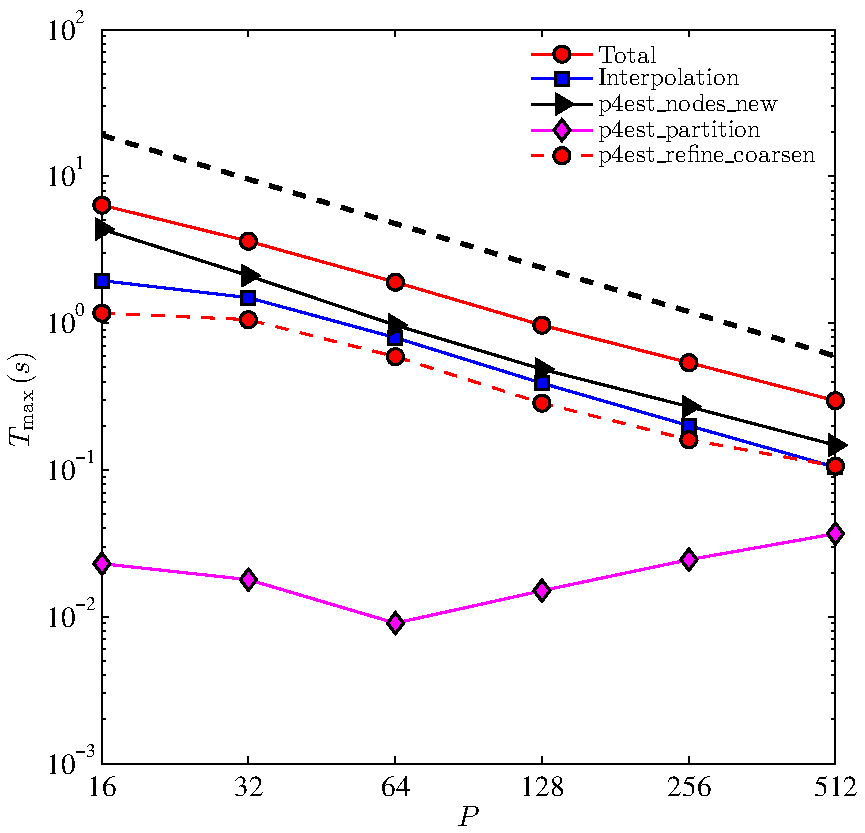
\includegraphics[width = 0.3 \textwidth] {figures/SL_Small_1_SemiLagrangian.pdf}}
		\subfigure[Semi-Lagrangian, $\text{CFL} = 10$]{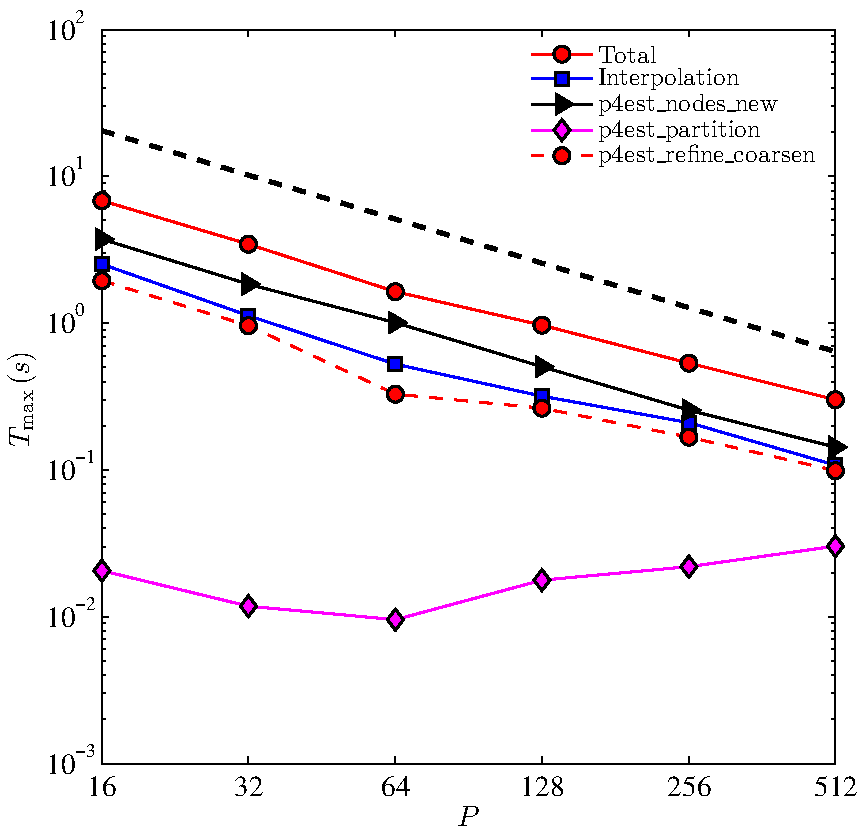
\includegraphics[width = 0.3 \textwidth] {figures/SL_Small_10_SemiLagrangian.pdf}}
		\subfigure[Semi-Lagrangian, $\text{CFL} = 100$]{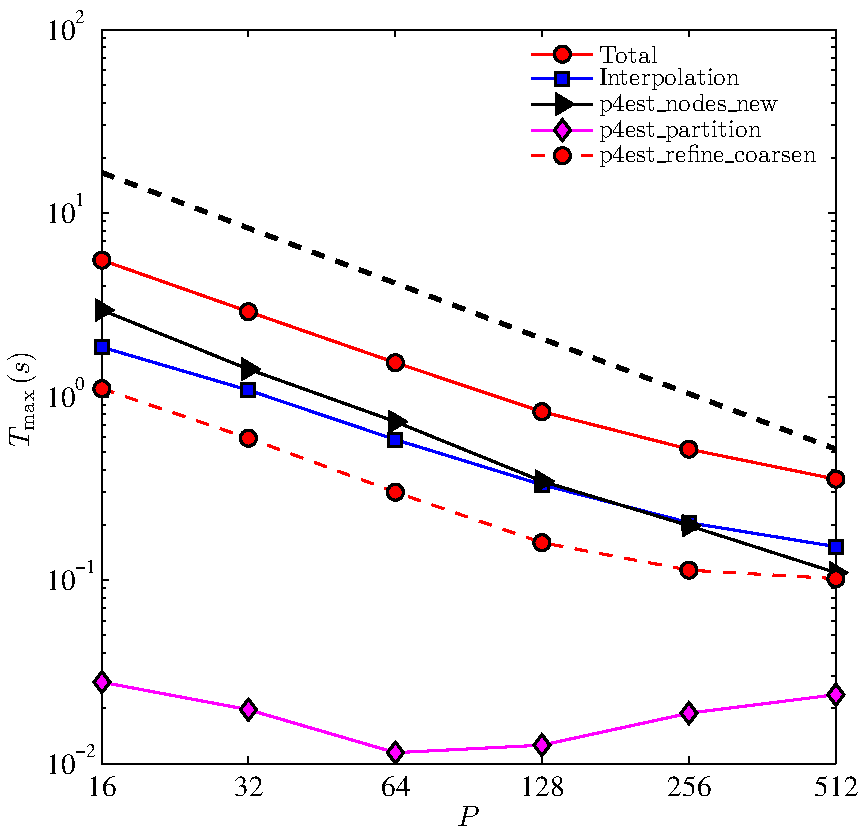
\includegraphics[width = 0.3 \textwidth] {figures/SL_Small_100_SemiLagrangian.pdf}}
		\\
		\subfigure[Interpolation, $\text{CFL} = 1$]{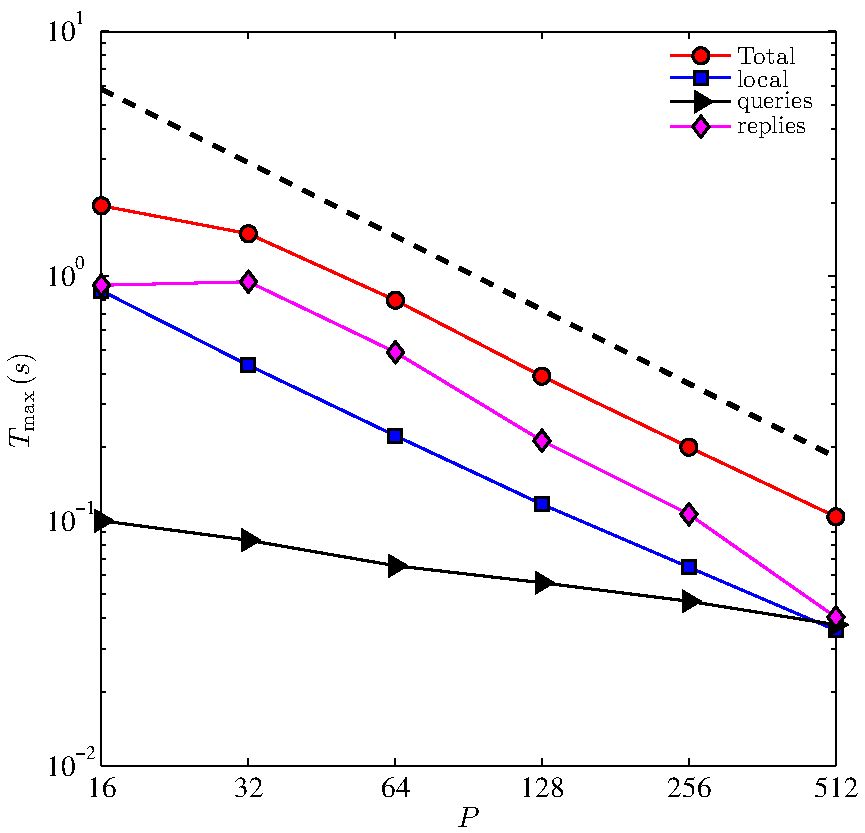
\includegraphics[width = 0.3 \textwidth] {figures/SL_Small_1_Interpolation.pdf}}
		\subfigure[Interpolation, $\text{CFL} = 10$]{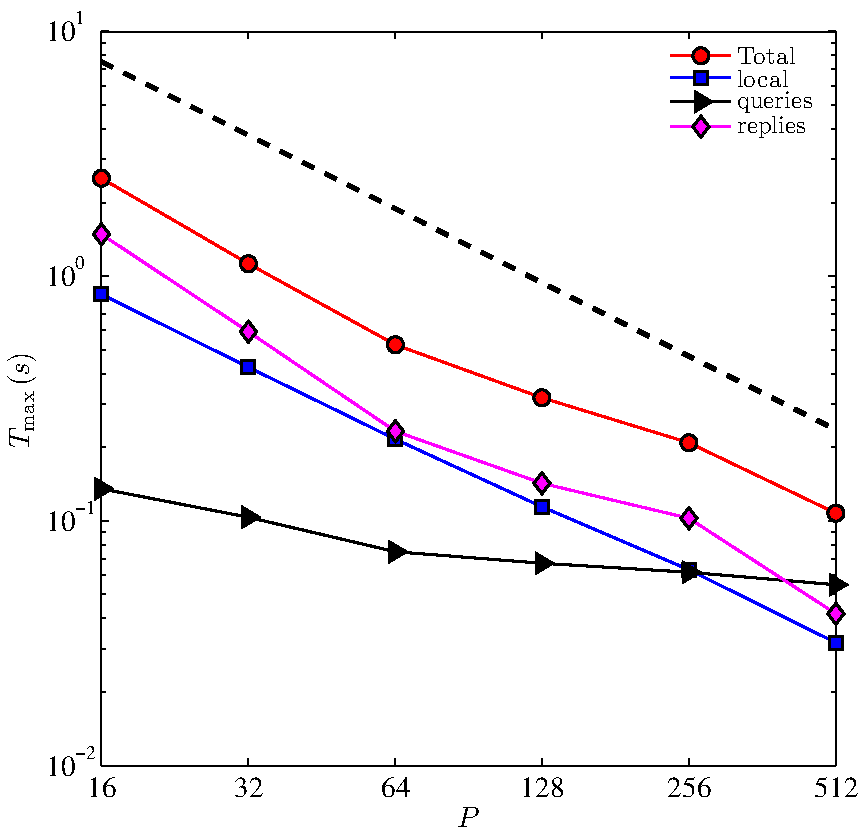
\includegraphics[width = 0.3 \textwidth] {figures/SL_Small_10_Interpolation.pdf}}
		\subfigure[Interpolation, $\text{CFL} = 100$]{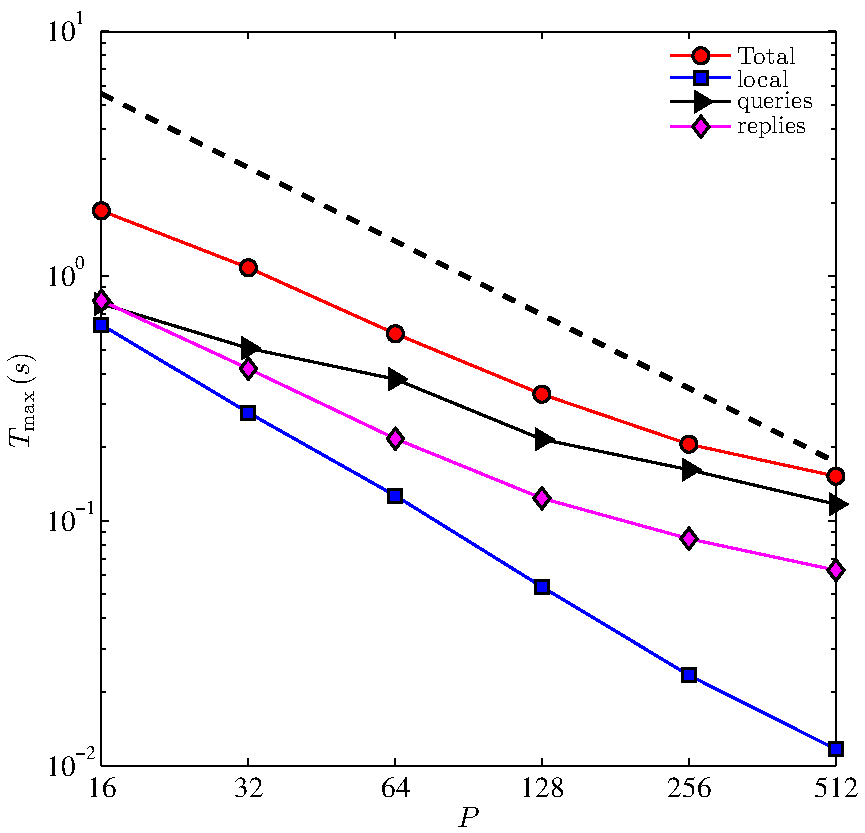
\includegraphics[width = 0.3 \textwidth] {figures/SL_Small_100_Interpolation.pdf}}
	\end{center}
	\caption{Strong scaling of a single iteration of algorithm \ref{alg:semi-lagrangian} for the rotation test on a level-10 octree with approximately 13M cells and 15M nodes. Top row: scaling of various components of the algorithm for (a) $\text{CFL} = 1$, (b) $\text{CFL} = 10$, and (c) $\text{CFL} = 100$. Bottom row: breakdown of various components of the interpolation phase for the same CFL numbers. Note that the maximum time has been scaled with the number of iterations required to build the tree (c.f. table \ref{tab:semilagrangian}).}
	\label{fig:semilagrangian_small}
\end{figure}

\begin{figure}[htbp]
	\begin{center}
		\subfigure[Semi-Lagrangian, $\text{CFL} = 1$]{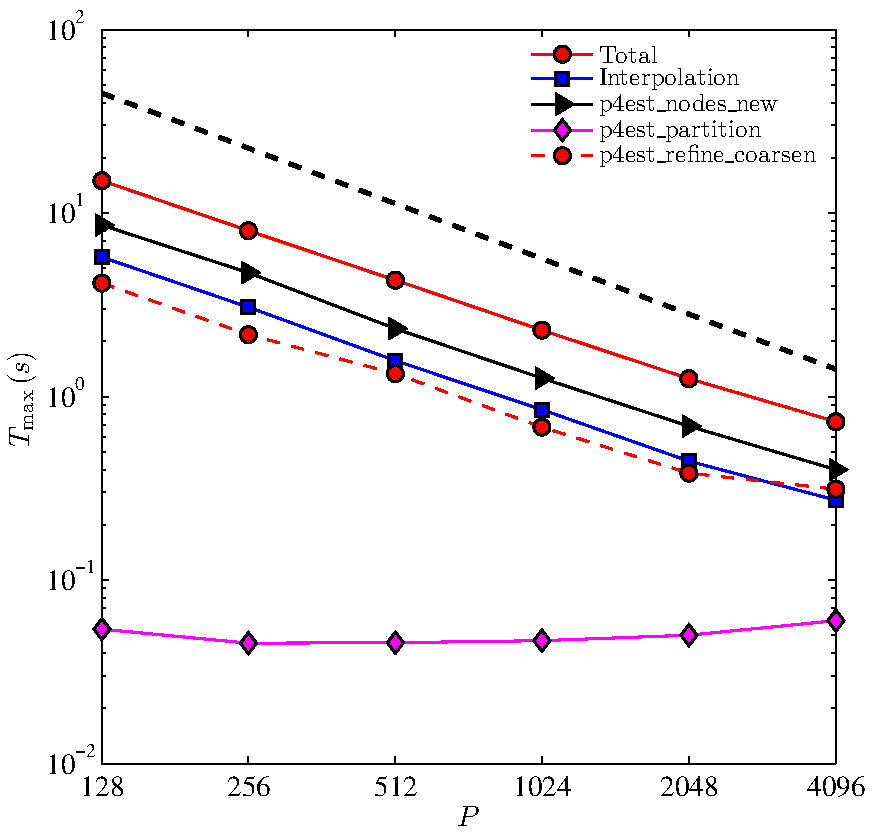
\includegraphics[width = 0.3 \textwidth] {figures/SL_Large_1_SemiLagrangian.pdf}}
		\subfigure[Semi-Lagrangian, $\text{CFL} = 10$]{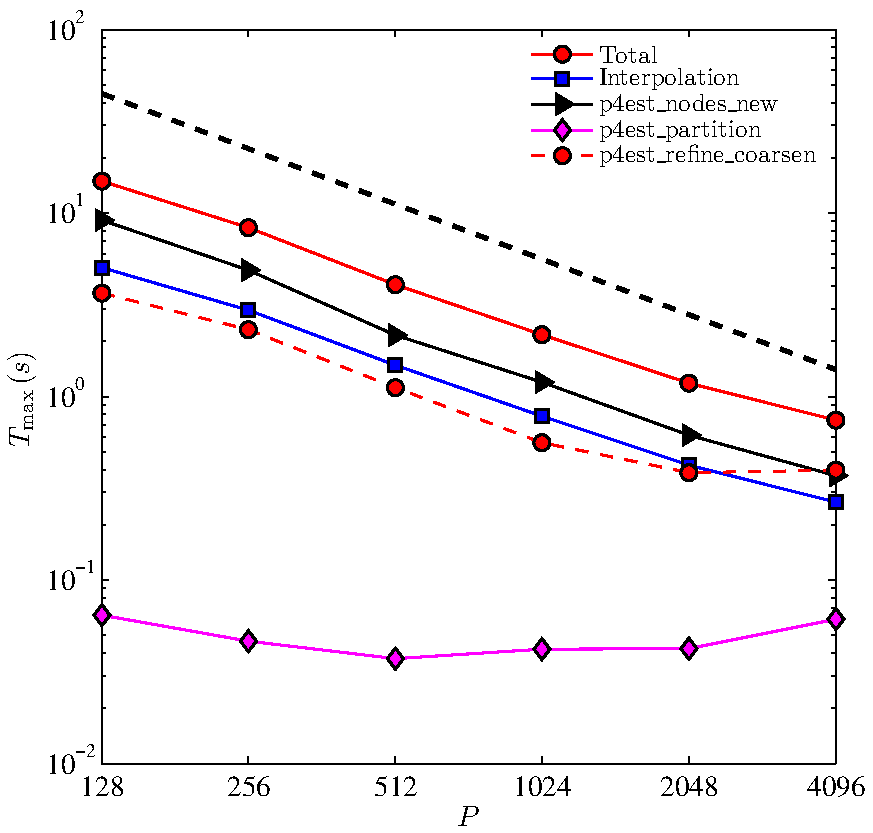
\includegraphics[width = 0.3 \textwidth] {figures/SL_Large_10_SemiLagrangian.pdf}}
		\subfigure[Semi-Lagrangian, $\text{CFL} = 100$]{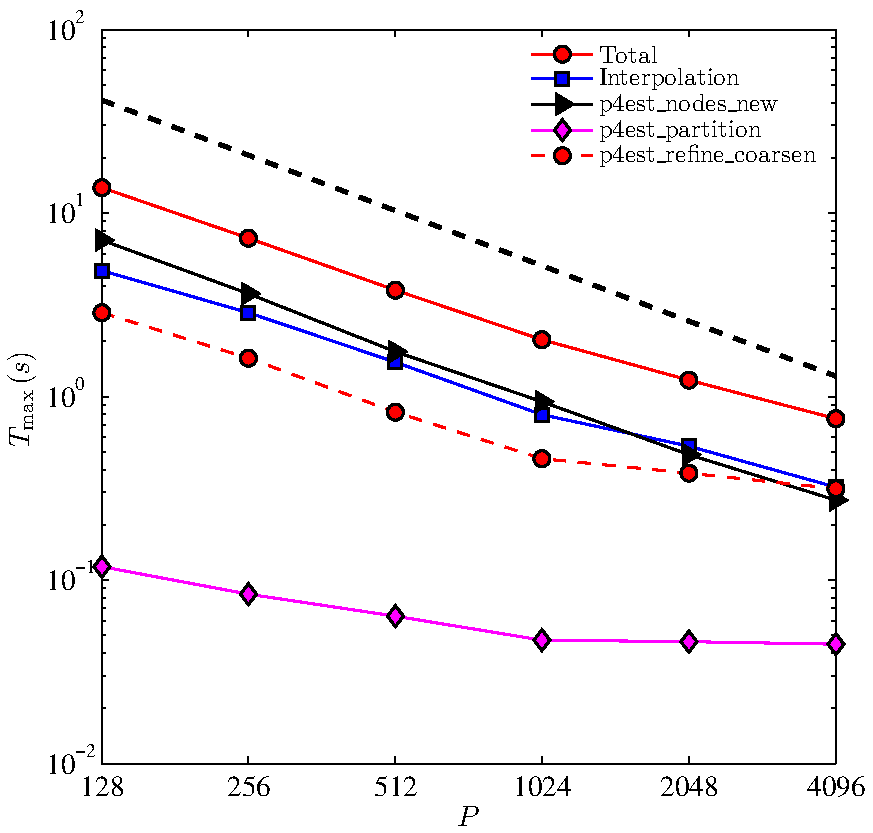
\includegraphics[width = 0.3 \textwidth] {figures/SL_Large_100_SemiLagrangian.pdf}}
		\\
		\subfigure[Interpolation, $\text{CFL} = 1$]{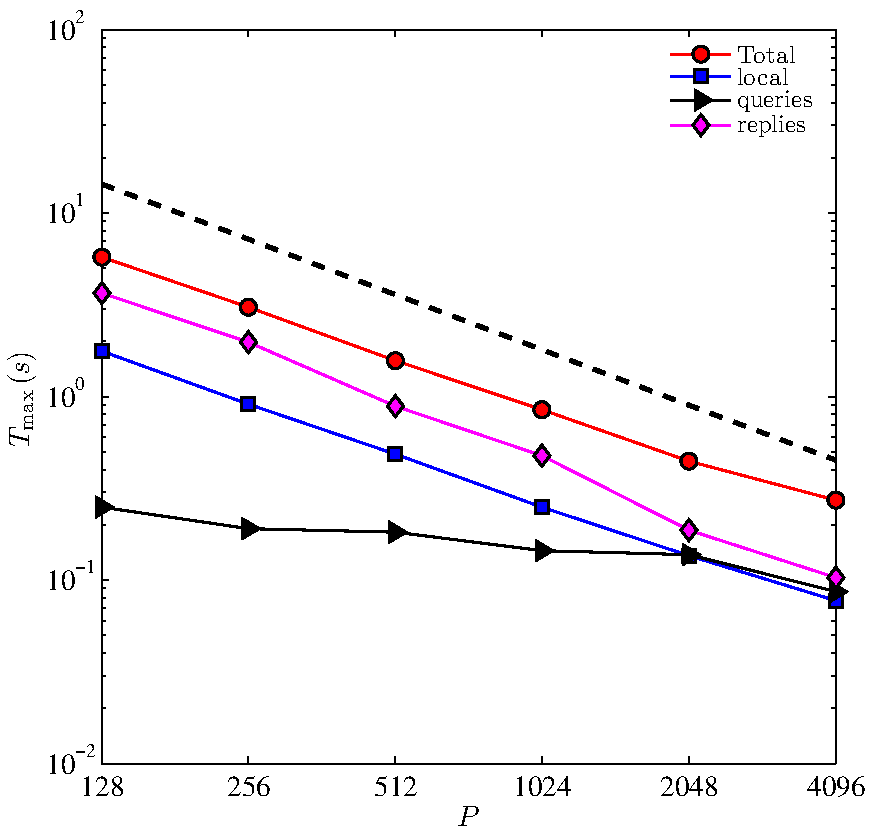
\includegraphics[width = 0.3 \textwidth] {figures/SL_Large_1_Interpolation.pdf}}
		\subfigure[Interpolation, $\text{CFL} = 10$]{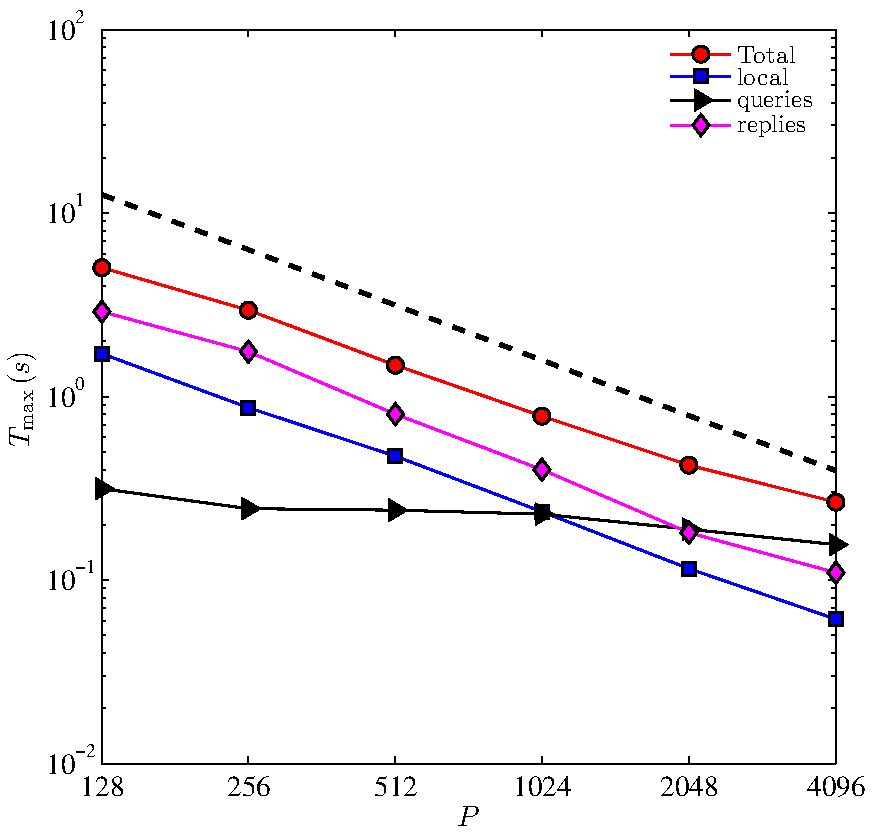
\includegraphics[width = 0.3 \textwidth] {figures/SL_Large_10_Interpolation.pdf}}
		\subfigure[Interpolation, $\text{CFL} = 100$]{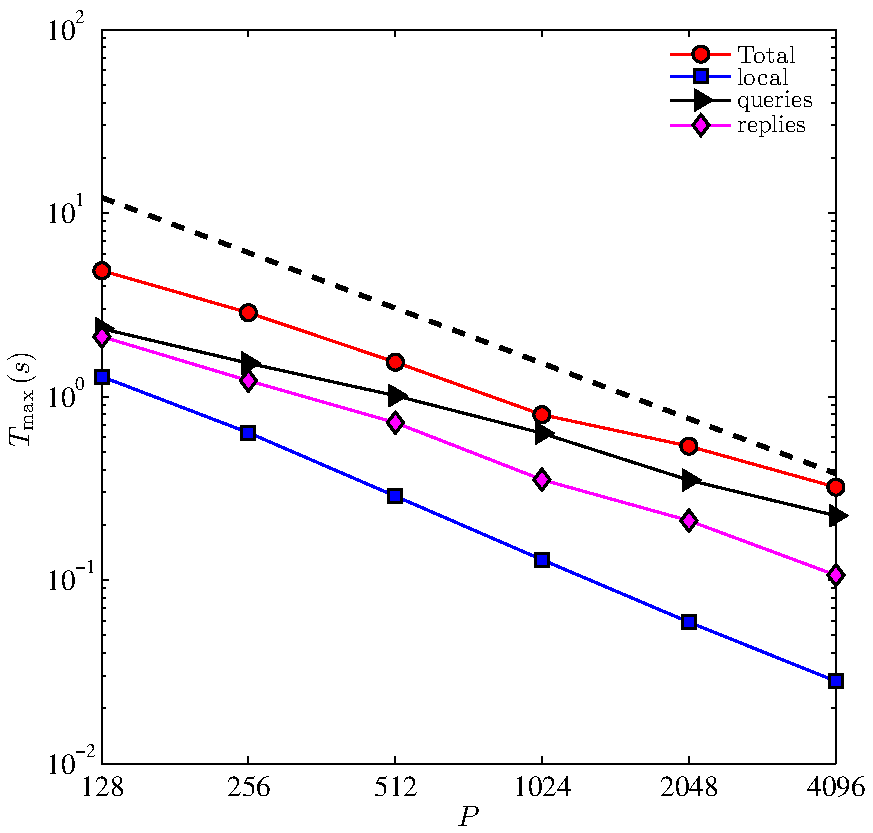
\includegraphics[width = 0.3 \textwidth] {figures/SL_Large_100_Interpolation.pdf}}
	\end{center}
	\caption{Strong scaling of a single iteration of algorithm \ref{alg:semi-lagrangian} for the rotation test on a level-12 octree with approximately 251M cells and 255M nodes. Top row: scaling of various components of the algorithm for (a) $\text{CFL} = 1$, (b) $\text{CFL} = 10$, and (c) $\text{CFL} = 100$. Bottom row: breakdown of various components of the interpolation phase for the same CFL numbers. Note that the maximum time has been scaled with the number of iterations required to build the tree (c.f. table \ref{tab:semilagrangian}).}
	\label{fig:semilagrangian_large}
\end{figure}

% \subsection{Reinitialization} \label{section::scaling_reinitialization}

% The reinitialization procedure presented in section \ref{section::reinitialization} necessitates the second order derivatives of the level-set function for the second order discretization in space. The finite difference schemes we implemented rely on the description of the neighborhood of each vertex in the adaptive tree environment. This information can either be computed on the fly or stored in a buffer. Fetching the neighbors information is rather time consuming and was observed to improve the overall scalability of the algorithm by increasing the local computation load. However, it slowed down the procedure significantly and therefore we choose to present the buffered version of the implementation. If one was to be limited in memory, constructing the neighborhood information on the fly would be a desirable option and would lead to better scaling, but in our case memory is not a limiting factor.

% The scaling results are presented in figure \ref{fig::scaling_reinitialization} and demonstrate satisfying scalability. Taking for reference the timing with $128$ processes, we observe efficiencies of $0.877$ with $1024$ processes, $0.763$ with $2048$ processes and $0.609$ with $4096$ processes.

% \begin{figure}[ht!]
% \begin{center}
% 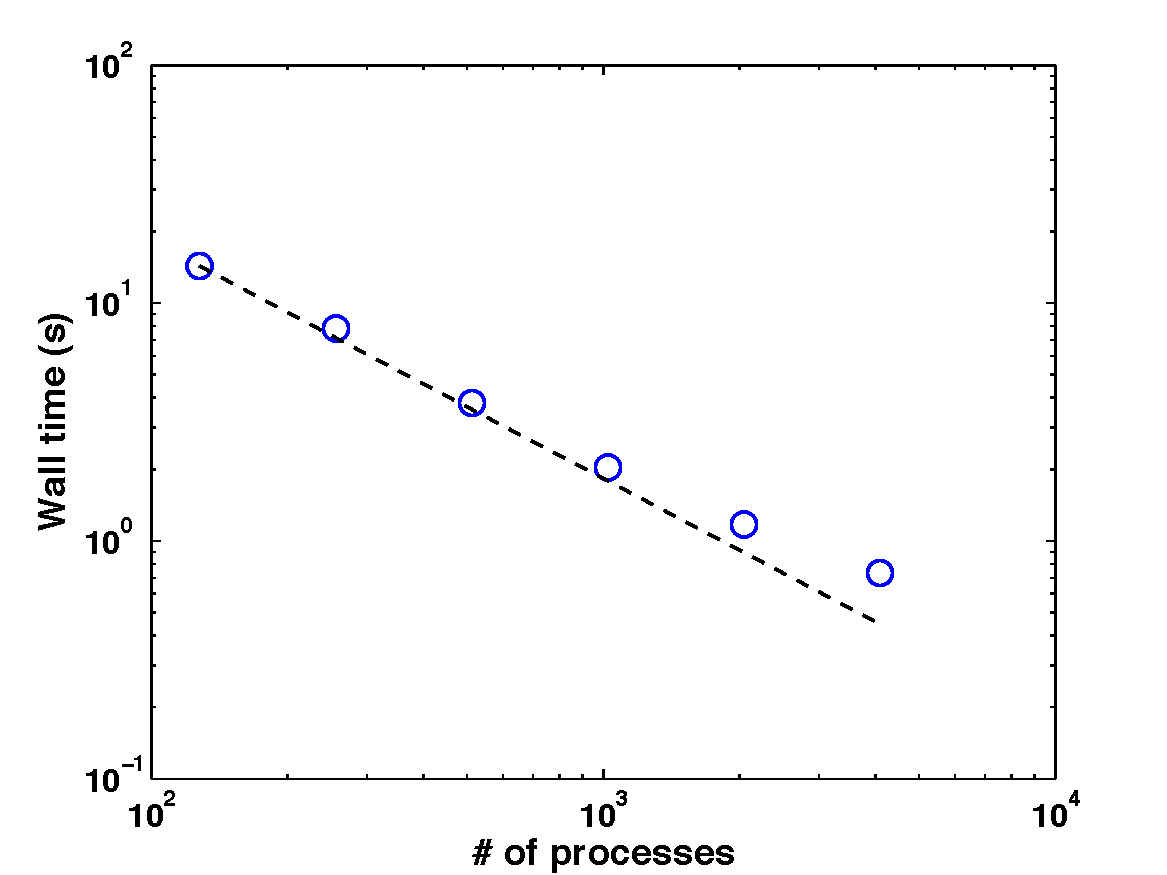
\includegraphics[width=.7\textwidth]{figures/scaling_reinitialization_1st_time_2nd_space_with_buffer.pdf}
% \caption{Scalability of the reinitialization procedure presented in section \ref{section::reinitialization} and analyzed in section \ref{section::scaling_reinitialization}.} \label{fig::scaling_reinitialization}
% \end{center}
% \end{figure}

% \subsection{Poisson solver}